%!TEX root = vaisagh_thesis.tex

\chapter{Literature Review}
\label{chapter:LiteratureReview}

Crowds are typically seen as a large collection of individuals sharing a common location and undergoing some common experience~\cite{Aveni:1997wq}. Depending on the experience being shared, individuals in a crowd can think, behave and react in different ways. In this thesis, the focus is on crowds involved in emergency egress. \emph{Egress} refers to the process of leaving a place, and emergency egress situations are situations in which a crowd tries to escape from danger due to fires, bomb blasts or other similar situations.

Crowd modelling and egress simulation are not \emph{new} areas of research in any sense of the word. A lot of researchers have worked on modelling and studying crowds and evacuations over the past few decades. These include psychologists, sociologists, computer engineers, civil engineers, etc. In fact, fire safety science is itself an active area of research with dedicated journals. In this chapter, the current state of research in the understanding and modelling of crowds and, more specifically, emergency egress simulation is introduced. A holistic approach is taken towards understanding and modelling the egress process through the examination of literature from all related fields. The objective of this holistic analysis is to determine the core components of the egress process and discover the steps in that process that can be investigated in this thesis.

 Section~\ref{LiteratureReiew:MultidisciplinaryNature} talks about the essentially inter-disciplinary nature of crowd simulation and the importance of understanding and utilizing the different viewpoints and approaches. Section~\ref{LiteratureReview:CurrentUnderstanding} introduces the reader to some of the psychological and sociological theories of crowds and people's reaction to fires. This helps determine the core processes that need to be considered in egress modelling and simulation. Subsequently, Section~\ref{LiteratureReview:EngineeringModels} explores the landscape of computational models of egress that have been developed over the years with a special emphasis on their ability to model the processes discussed in Section~\ref{LiteratureReview:CurrentUnderstanding}. This helps motivate the rest of the thesis.

\section{Multidisciplinary Nature}
\label{LiteratureReiew:MultidisciplinaryNature}

A complex system can be defined as a system with many interacting entities whose properties are well defined. Inequalities in spatial and temporal interactions at the microscopic level can lead to emergent macroscopic phenomena~\cite{Sloot:1997ws}. An emergency egress simulation is just such a complex system with a lot of interacting elements. This system is made of a large number of human beings, the building, fire, smoke, fire alarms and other entities which might be specific to the location or type of emergency. Besides physicists studying the physics behind the development and spread of fire and smoke, there are other scientists and engineers who work on computationally modelling the spread of fire or smoke and the different complexities involved. There are also fire safety experts who work on improving the effectiveness of fire alarms and PA systems and, in general, on improving the efficiency of egress. A lot of researchers also work on the element at the core of this complex system: crowds or, more generally, human beings.

Many psychologists have been studying crowds and how individuals behave in crowds for over a century now and many theories have been developed. A lot of these theories contradict each other and there is generally little consensus on which is the best. Torres~\cite{Torres:2010tj} provides an excellent comparison of the different existing theories of crowd behavior. He does so by comparing their effectiveness in explaining the fire that occurred at the Station night club in West Warwick, United States on Feb 20, 2003. Section~\ref{LiteratureReview:CurrentUnderstanding}, which presents and explains some of the existing crowd behavior theories, uses the findings from this thesis extensively.

How people interact with each other and act in a crowd is just one aspect of the person's behavior during a fire. For instance, people don't start evacuating the building as soon as they hear an alarm or as soon as they hear there is a fire. Each \emph{cue} that he/she observes has a certain impact on the person depending on his/her identity, social role and the circumstances. There are a lot of studies~\cite{Kuligowski:2009un,Ozel:2001tn,Torres:2010tj,Pires:2005gs,Sime:1983uy} that examine the effect of different cues on egress behavior and the other aspects of what we refer to as \emph{pre-evacuation behavior}. Kuligowski~\cite{Kuligowski:2009un} presented a list of various cues and how each of them affects a person. She emphasizes how cues need to be perceived and interpreted and how the decision for an action is taken based on these cues.

How decisions are made is itself an active area of research. Besides the theories on crowd behavior, some studies~\cite{Pires:2005gs, Ozel:2001tn}, also propose different ways in which humans make decisions during emergencies. There are also several other dimensions to understanding the behavior of individuals engaged in egress. Various studies~\cite{Andree:2008td,Sandberg:1997tw,Kobes:2009jx} discuss the effects of culture on egress and others~\cite{Pelechano:2005vp,Aydt:2011wz} propose detailed models of emotion.

Computational models of egress try to model and simulate a crowd engaging in emergency egress so that these situations can be effectively tackled. There are several different computational models of egress and each of them have their own advantages. The major difference in opinion among computational model developers is on the amount of abstraction to be used. Some models like network based models and flow models, do not explicitly consider humans but rather view crowds as a homogeneous entity. These approaches are simpler for the modeler and computationally less resource intensive. Despite this, some crucial details like flow rate through doorways and the rate of survival can be approximately measured and analyzed. Agent Based Models, on the other hand, use significantly lesser abstraction in modelling crowds and are thus capable of simulating the heterogenity in crowds. These approaches take a bottom up approach; by specifying each individuals behavior it can more accurately approximate real life behavior. There are also more detailed agent based models of egress simulation that model human memory and emotions. These different modelling techniques and models and their strengths and weaknesses will be discussed in more detail in Section~\ref{LiteratureReview:EngineeringModels}.

Some studies~\cite{Torres:2010tj,Sime:1995uu,Aguirre:2004tn} criticize computational models made by engineers and computer scientists for not taking into account the considerable advancements in the understanding of human behavior made by psychologists and sociologists. Recently, some models~\cite{Pan:2006vp} have made a start in this direction by recognizing the need for behavioral models. However, despite being about two decades old, Sime's quote~\cite{Sime:1995uu}:
\begin{quote}
To date the significance of human cognition, decision making and social behavior seems to be recognized, but has not been fully incorporated into the prototype working models \ldots
\end{quote}
on behavior models is still very much applicable as will be illustrated in the following pages.

For example, the idea of panic or \emph{non-adaptive behavior} is at the center of several behavioral models~\cite{Pan:2006vp,Franca:2009wq}, but studies have shown that this concept is neither clearly explained~\cite{Torres:2010tj} nor well accepted~\cite{Cocking:2005uc,Paulsen:1984ti,Proulx:2001we,Ramachandran:1990wj,Sandberg:1997tw,Sime:1995uu}. Also, it is difficult to find computational models that model factors like \emph{pre-evacuation behavior} and \emph{incomplete knowledge} of evacuees.

As our knowledge of human behavior, emotion, social interactions and decision making expands, a more complex picture of human behavior has been emerging. The use of this knowledge in egress modelling has been limited. With current advancements in technology, there are fewer reasons to make unnecessary abstractions; thus, higher fidelity models of egress can be developed. With this purpose, the next section gives an overview of the current state of knowledge about human behavior in crowds and emergency situations.

\section{Current Understanding of Human Behavior During Egress}
\label{LiteratureReview:CurrentUnderstanding}

As discussed earlier, a fire evacuation is a complex situation to model and simulate. The main reason for this complexity is that the system has a complicated entity at its center: a thinking, feeling and socializing human being. To accurately simulate the evacuation of a building in an emergency situation, it is necessary to understand the behavior and decision making of the people taking part in it. As briefly mentioned in Section~\ref{LiteratureReiew:MultidisciplinaryNature}, there are a lot of conflicting views and theories on how humans behave in emergencies and why they behave as they do. However,  there are certain behaviors that are fundamental to human nature and are generally accepted as fact like the tendency to search for familiar surroundings~\cite{Mawson:2005tq,Paulsen:1984ti,Ramachandran:1990wj,Sandberg:1997tw} and the constant search for information~\cite{Proulx:2003tc,Tong:1985wn,Ozel:2001tn,Sime:1983uy}. In this section, the reader is introduced to some of the major accepted ideas on the nature of human behavior during egress and some of the major theories on the same.

\subsection{Pre-evacuation behavior}
\label{LiteratureReview:HowItAllBegins}

In an ideal scenario, all occupants on hearing a fire alarm, use the nearest safe exit to leave the building. However, this is hardly the norm. In most cases, occupants are used to hearing false alarms and often do not start to evacuate until they are completely sure that it is needed. On January 19, 2000, a fire in Boland Hall in Seton Hall University in United States killed three students because they had ignored the fire alarms assuming they were false alarms~\cite{Berry:2000us}. This uncertainty about the authenticity of a first sign of danger isn't an isolated incident~\cite{Graham:2000vl,Proulx:2001we,Proulx:1995wq,Proulx:2003tc,Purser:2001ts,Ramachandran:1990wj,Sime:1995uu,Tong:1985wn}. So, when studying the behavior of evacuees, it is necessary to study and understand their actions right from the point the fire started~\cite{Tong:1985wn} rather than the time at which they start evacuating.


During an emergency there are some changes in the environment that indicate that something is wrong or different from normal. These changes are called \emph{cues}~\cite{Sime:1983uy}. Broadly, cues can be categorized as \emph{ambiguous} and \emph{unambiguous} cues depending on the clarity of the signal sent to the evacuee. For example, hearing noises is ambiguous, while seeing smoke or fire is unambiguous. Cues and their effects will be discussed in more detail in Section~\ref{PreEvac:LitRev}. The following paragraphs give a brief summary of the discussion to give a broad idea of pre-evacuation behavior.

Several studies~\cite{Ramachandran:1990wj,Proulx:2007ul,Tong:1985wn} have discussed the effect of ambiguity of cues. Most importantly, cues have to persist for a period of time before evacuees even initiate investigation which can eventually lead to evacuation if more information is found. There are several factors that influence the effect of the cue on an evacuee. This includes the evacuees intrinsic factors like age and gender. In a classic study~\cite{Latane:1969wm}, participants where placed in a room with smoke for a period of time in two different situations. The experiment showed that when alone, 75 percent of the subjects reported the smoke. In the presence of two non-reacting others only 10 percent of the subjects reported the smoke during the experimental period. People react differently to fires depending on their familiarity with the environment and preparedness for the emergency~\cite{Proulx:2003tc,Proulx:2001we,Paulsen:1984ti,Sandberg:1997tw,Cocking:2008vv,Tong:1985wn}.

In general, the term \emph{pre-evacuation} refers to the period of time that elapses between the start of the fire alarm (which is generally the first cue) and the person starting egress. According to several studies this process can itself be broken down into three sub-processes:

\begin{enumerate}
	\item Perception: The fact that a cue exists does not mean that the evacuee has perceived it. For example, he could be asleep.
	\item Investigation: Once some cues are perceived, evacuees start an investigation process that may consist of milling or simply exploring (Section~\ref{LiteratureReview:CrowdBehavior}).
\end{enumerate}

It's only once investigation reveals sufficient information to warrant an evacuation that evacuees start evacuating. It is a general misconception that people panic and stop acting rationally as soon as they see a situation like a fire. Several studies~\cite{Kobes:2009jx,Schadschneider:2008cz,Reicher:2008ep,Torres:2010tj,Paulsen:1984ti,Sime:1983uy} have disproved this claim. Irrational panic is hardly ever the standard first reaction to seeing fire. Rather, people react rationally and try to gain more information so that they can act in a manner more appropriate to the situation.

This section presented the literature on how the process of evacuation starts. The process called \emph{pre-evacuation} consists of two phases: perception and interpretation. Cues present in the environment indicate to the evacuees that there is something happening in the environment. These cues can be of different types and their effect varies based on certain factors of the environment and certain characteristics intrinsic to the evacuee. During the second phase people search for verification that the situation does indeed require some action and various cues and other factors help him towards this realization.  % Concluding line to give a continuation to the next subsection.

\subsection{Crowd behavior}
\label{LiteratureReview:CrowdBehavior}

% In the previous section, the effect of groups on cue perception had been briefly discussed. Groups actually have a much more important role to play in evacuation than just being a factor that influences cue perception. Each human is not an isolated individual. Being a social being, he is influenced by the people around him, even when they aren't actually his companions. As stated by Tong and Canter~\cite{Tong:1985wn}:

% \begin{quote}
% Research on human behaviors in fires reveals the dynamic process actors engage in to deal with an emerging threat. Emergency egress is a complex social process; it is false to assume humans automatically take protective measures upon hearing an alarm or notification that a threat is present in their environment.
% \end{quote}

This section discusses different theories of crowd behavior that, in general, deal with the phase that commences after \emph{pre-evacuation}. According to Tong and Canter~\cite{Tong:1985wn} emergency egress is a \emph{complex social process}. What this complex social process is, has generally been a matter of much debate with a great deal of conflicting theories on the same. In his PhD thesis~\cite{Torres:2010tj}, Torres categorizes the theories on crowd behavior into six:

\begin{itemize}
\item {\bf Social Breakdown Model}: According to this theory, a fire evacuation is characterized by competitive behavior~(pushing and shoving). As competition develops traffic jams occur at the doors or passageways. This competitive behavior is because the individuals think only about getting themselves out without concern for the other trying to escape, low optimism and a large group size which makes people think that they need to push and shove to stay alive. This model suggests that the reason for deaths and problems during egress is because of \emph{non-adaptive behavior}. Non-adaptive crowd behavior is the type of crowd behavior that does not adapt to an emergency situation and often leads to destructive consequences.

\item {\bf Hysterical Belief Model }: This model is also characterized by flight and non-adaptive behavior. However its cause is slightly different. In this model, it is necessary for a collective belief in a generalized threat to develop before people start panicking. This belief in a generalized threat, develops when people perceive ambiguous cues and then feel anxious due to certain factors, like a feeling of reduction in exit choices; this, in turn, leads to a feeling of unambiguity in believing in a generalized threat which they can counter by fleeing. Also certain \emph{components of social action} need to have been completed that permit panic to occur. These components are characterized as being actions that are as per norms~(i.e. not non-adaptive) and which are done for the benefit of the entire crowd or collective. Emergent norm theory can be considered to be a kind of hysterical belief model. According to this, there is an extended period of \emph{milling} during which people engage with others and exchange experiences. During this period a consensus develops and leaders also develop. Everyone in the group follows the actions of the leader in a process referred to as \emph{keynoting}.

\item {\bf Non-Social Model }: This theory's main proponent is Quarantelli~\cite{Quarantelli:1954vr}. According to this theory, people largely act in a pro-social manner; yet there occurs a point where a collective threat becomes severe and conditions emerge where social bonds break down and actions designed for self preservation emerge. The key point of difference from the previous models is the importance given to social bonds and the association of flight or competitive behavior or panic with breaking of these social bonds~(this is a necessary but not a sufficient condition). Also competitive behavior is associated with individuals and not the group as a whole as specified in the hysterical belief model. As above, a perception of dwindling number of exits is also a precondition.

\item {\bf Normative Model }: This model is characterized by people helping one another during the emergency egress and an overall lack of competitive behavior. This theory is also characterized by a tendency to fight fire.

\item {\bf Affiliative Model }: This model conceptualizes emergency egress as people engaged in stimulation seeking behavior by moving towards others they feel close to or running towards locations that are familiar. People are assumed to have cognitive maps and a cue triggers a tendency to try to restore congruity to their cognitive map. People seek familiarity to such an extent that they might even move towards a threat. Even competitive behavior is affiliative in nature, i.e., people try to exit with their primary groups rather than alone~(as in the non-social model). This search for familiarity might manifest itself as a search for group members or in other cases as taking a familiar route or in others just moving towards locations that are familiar.

\item {\bf Self Categorization Theory }: In this model, the people's groups aren't fixed. They tend to develop a sense of `we-ness' with others present in the evacuation. Drury et al.~\cite{Drury:2009ga} showed that collective bonds may be strengthened and even created through the experience of an emergency. This is characterized by people helping strangers escape. This dynamic emergence of groups was also observed by several others~\cite{Aveni:1997wq,Reicher:2008ep,Cocking:2007wp,Cocking:2008vv}. When part of a group, people tend to follow the group consensus. Leaders develop for groups and these leaders can impose their will on the group. Groups that are formed are highly dependent on context and other groups and in turn the individuals present. Groups aren't static, they have dynamic characteristics. When faced with an adversity~(like a fire), behavior in a group reaches a common level with time. The elaborated social identity model~(ESIM) for crowds was an extension to this theory proposed by Reicher~\cite{Reicher:2008ep} which proposed an even more dynamic model of social identity and group behavior where the social role or identity of an individual can be influenced by his actions and vice versa.
\end{itemize}

Tong and Canter~\cite{Tong:1985wn} stated that there are three distinct strategies that people adopt in a fire, the first of which is to~(try to) extinguish the fire, the second is to seek shelter and wait to be rescued and the third is evacuation. Most of the theories state that people engage in flight behavior, i.e.\ they attempt to escape rather than fight the fire. Only the normative model predicts a fire fighting behavior and this kind of behavior was shown by only 4 of the people surveyed by Torres. It is interesting to note that in over three quarters of the domestic fire incidences that occurred in the United Kingdom and Australia, the fire was extinguished either naturally or by the residents; fire fighters were not called~\cite{Kobes:2009jx}. However, as further highlighted in the same paper by Kobes et al.~\cite{Kobes:2009jx} there is very little literature on fire fighting behavior shown by occupants besides this. This might be because of a difference in attitudes towards private and public property. Nevertheless, there is not enough evidence to show that fire-fighting is normally done by occupants. This, however, does not suggest an absence of altruistic behavior. Other models like the affiliative model and SCT model do suggest that people do show altruistic behavior in helping others who are part of their group or who they characterize as being part of their group.

All the models predict that as long as people are capable of escape, they try to escape; and panic is not an influential factor. The chart shown in Fig.~\ref{fig:EgressAge}~(obtained from~\cite{Klupfel:2005to}), shows the relationship between mobility, complexity of the architecture and people's reaction to fire. This chart indicates how, unless forced to, people do not defend in place or try to find refuge. It also confirms the preference for familiarity~(of a refuge) to staying in place and defending against the fire. The fact that people always try to escape and rarely seek shelter even in the case of extreme smoke has been confirmed by Kobes et al.~\cite{Kobes:2009jx}.

\begin{figure}[!t]
\centering
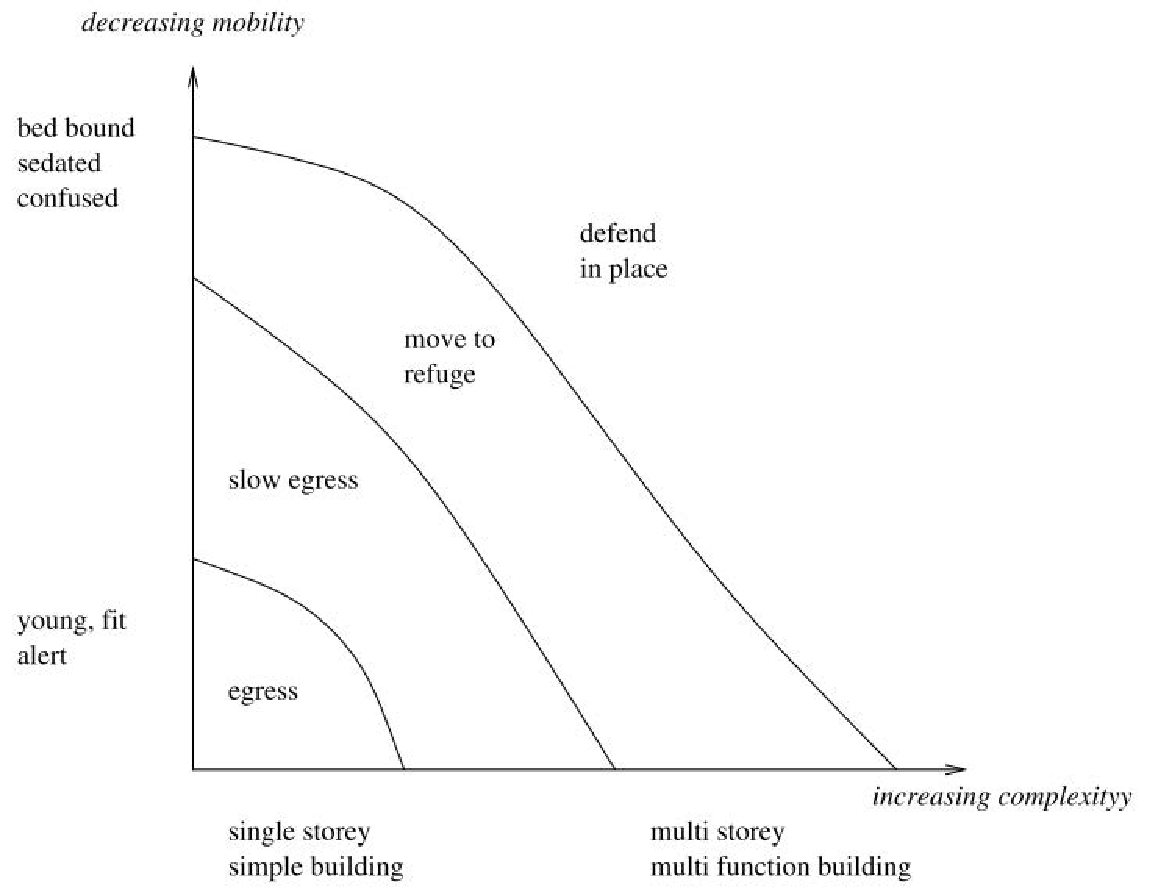
\includegraphics[height=4in,width=\textwidth]{LiteratureReview/EgressStrategies}
\caption[Strategies for Egress]{According to this chart from~\cite{Klupfel:2005to} there are four strategies that humans resort to in egress. Studies have shown though that more often than not, egress or slow egress are the only strategies taken.}
\label{fig:EgressAge}
\end{figure}

However, it is important to note that flight behavior is not equivalent to competitive behavior characterized by pushing and shoving. The competitive behavior, which is central to the first two models listed above, has been established to be non-existent during egress, at least not in the sense of it spreading through the crowd. Cocking and Drury~\cite{Cocking:2005uc}, who are the main proponents of the self categorization theory, do admit that individual panic does occur; but rather than the panic spreading through the crowd it is the calm people who manage to impose their will on other people and calm the people who panic. The same thoughts were echoed in other studies~\cite{Paulsen:1984ti,Sime:1983uy,Schadschneider:2008cz}. Several studies~\cite{Sime:1983uy,Paulsen:1984ti,Drury:2009ga} actually take a much stronger stand that competitive behavior almost never happens and rather people almost always behave altruistically. This was further confirmed by Torres~\cite{Torres:2010tj} who found that individual competitive behavior never occurred. Nevertheless, people did do whatever they could to enhance their and their group's survival but without knowingly causing harm to others~(which is what competitive behavior/ panic entails).

A further point in favor of the latter four models is the importance that they give to social bonds. For example~\cite{Cornwell:2003uo,Chertkoff:1996vw,Andree:2008td}, among others, have already demonstrated the important role that familiarity plays in behavior during egress. This was reaffirmed by Torres~\cite{Torres:2010tj}, who found that even in cases of extreme danger, people still maintained their social bonds. In fact, as opposed to the non-social model, in the real life evacuation, social bonds never broke down. If people did manage to get out of the fire, they would try to come back or help their trapped group members in some way~\cite{Torres:2010tj,Kobes:2009jx}.

The normative model, affiliative model and the SCT models also recognize the importance of social roles in determining the reactions of people to fire. Several studies have made this observation~\cite{Proulx:2003tc,Proulx:2001we,Paulsen:1984ti,Sandberg:1997tw,Cocking:2008vv,Tong:1985wn}. These models explain how the employees of a workplace who are trained or prepared, generally try to guide customers to the closest exits. They also indicate that within groups, the leaders or caregivers~(e.g.\ teachers or parents leading a children) continue to take the role of leaders during egress and try to find safe evacuation paths to protect their group.

% Another important point to be noted is the importance of inter group and intra group interactions and how these interactions affect the decisions and behaviors of the individuals in them. The emergent norm theory explains these through a process of milling and keynoting. While this theory can explain many situations, there are certain problems with this approach which are explained quite well in~\cite{Reicher:2008ep}. The most notable of this is regarding the extended period of milling that is proposed to take place regardless of time constraints. The current understanding~\cite{Reicher:2008ep} is that each person has an individual identity and a group identity. The group identity and the individual identity are highly interconnected in the sense that each individual influences the group's behavior and vice versa. Whileleaders in groups are important, it does not support the idea of keynoting where only the leader has full power over the group.

In summary, most experiments and studies have been in favor of an affiliative or SCT based model with certain elements of the normative model included. The consensus is that people always try to escape while trying not to compete with each other and they look for familiar people or locations in dangerous situations and if possible they even form new bonds with strangers stuck in similar situations. Also, the social role of a person determines his behavior. Staff try to ensure safe egress of customers and social leaders~(parents, teachers, etc.) take more responsibility during these times. Irrationality of occupants and panicking crowds are some of the common themes running through news reports of fire incidents. This discussed in more detail in the next section.

\subsection{On the rationality of crowds}
\label{LiteratureReview:RoleOfStress}

 It has been shown~\cite{Kobes:2009jx,Schadschneider:2008cz,Reicher:2008ep,Torres:2010tj,Paulsen:1984ti,Sime:1983uy} that very rarely do people panic and behave irrationally in spite of time constraints and stress. However, situations have been observed where people do not take the best possible actions and do not act in their best interests~\cite{Sandberg:1997tw}. This is probably because a person's rational thinking is bounded by the constraints of his/her knowledge of the environment i.e.\ he/she is only bounded rational. Bounded rationality is an idea that is becoming increasingly popular in behavioral economics and it implies three major things~\cite{Jones:1999tn}:

\begin{enumerate}
\item People do not know everything.
\item People cannot think infinitely into the future. They think in the short term and tend to take decisions that benefit them in the short term.
\item People are generally loss averse i.e.\ they do not like to take a risk of loosing more even if the gains are much higher. In a fire evacuation this means that people avoid action for small problems and take drastic actions as things get out of control. This is because early action might result in huge losses~\cite{Graham:2000vl}.
\end{enumerate}

If they are only bounded rational and they tend to make worse decisions as the fire gets worse, then it implies that the time pressure and stress must play some part. Ozel~\cite{Ozel:2001tn} proposed a decision making theory which explains this. The basic premise of his theory is that given the same set of information, people may attend to information differently depending on the stress and amount of time pressure they experience. When people gain information they feel less stressed. This can also explain why people investigate and try to gain more information when they perceive the first few ambiguous cues of fire.

One of the significant ideas suggested by Ozel~\cite{Ozel:2001tn} is the idea of filtration. According to this, to cope with time pressure and unavoidable conditions, people try to filter out all the cues that they deem as unimportant or less important. The rate of this filtration increases as the time pressure increases and as a result cue utilization decreases. This in turn implies that they have lesser information about the environment and tend to behave less rationally. This effect has also been observed by Davis et al.~\cite{Davis01122009} in older people who, due to age, are only able to process less information. The significance of information in egress and more particularly perception will be discussed in more detail in Chapter~\ref{chapter:IBP}.

Thus it is understood that humans act rationally within the bounds of their knowledge. However, as the situation worsens, their behavior tends to look more irrational to an observer. This is because the evacuees observe less on being stressed and as a result have lesser knowledge; this subsequently results in, what appears to be, irrational actions.

\subsection{Summary}
\label{LiteratureReview:PsychSummary}

The previous pages of this thesis have discussed the existing understanding on human behavior during egress through the analysis of incident reports, experimental studies and other reports in a wide number of fields. Several features of human behavior during egress that could play a key role in ensuring safe egress were discovered through this analysis. These are briefly summarized below:
\begin{itemize}
\item Ambiguous cues: Most cues are ambiguous in nature and they need to be present for a certain period of time before catching someone's attention enough for them to even start investigating.
\item Early investigative behavior: Early movement is characterized by investigation rather than egress. The investigators then gain knowledge or information either from what they observe directly or from what they hear from others. So there is a \emph{spread of information} in the environment~\cite{Fahy:2010to,Purser:2001ts}.
\item Flight behavior: Once people interpret the situation as fire, they react to it by trying to get out of the building. They do not try to fight the fire or to seek shelter unless they are forced to by the circumstances.
\item Search for familiarity: People's first action while trying escape is to move around and try to find their primary group members who they are familiar with. They then try to exit through some exit that they are familiar with rather than observing new signs. The search for familiarity, also implies the importance of groups and social bonds, to the extent that even after exiting the building, people might come back to help people from their group.
\item Absence of competitive behavior: People do not engage in competitively pushing or shoving others when engaging in egress. The rare cases when pushing or shoving occurs, it is because the individual involved is forced to do so.
\item Altruistic behavior is common: People tend to help others who need help. They also do not panic or act irrationally. Instead, they follow social norms and try to be as orderly as possible.
\item Decisions and behaviors are dynamic: As people interact with the environment and the other people in the crowd their decisions and behavior might change or be influenced.
\item Bounded rationality: Stress and time constraints cause a reduction in cue utilization and information availability and thus cause people to make decisions that with complete information will seem irrational.
% \item Groups are important: Groups and social bonds form an important part of determining the person's behavior and decisions. People within a group exchange information and groups also pass on information to other groups. Each group then makes decisions based on the groups intrinsic properties and the information available to them which in turn is determined by the characteristics of the individuals who make up the group. Most groups also have a leader who takes the lead in trying to make decisions.
\end{itemize}

The next section presents an analysis of existing approaches to computation modelling of egress. These models are analyzed against the understanding of human behavior that has been presented in this section. This helps in identifying the research problems that are tackled in the rest of the thesis.

\section{Computational Models of Egress}
\label{LiteratureReview:EngineeringModels}

Conducting experiments and analyzing an environment or an event for its safeness can be expensive and, more importantly, quite dangerous. Through modelling and simulation,  it might be possible to prevent the unnecessary loss of life. It can help architects design buildings better and the management and fire fighters to handle situations better. These models have to be able to accurately simulate how humans behave in order to be useful. A good predictive model can also help test the existing theories of human behavior through the study of emergent behavior. In the previous section the reader was introduced to psychology and sociology literature on how humans and crowds behave in fire and other evacuation scenarios. In this section, computational models of egress that have been developed over the years will be discussed. Section~\ref{LiteratureReview:ComponentsOfAModel} introduces the different components that generally constitute a computation model of egress. Section~\ref{LiteratureReview:ExistingModelsSummary} presents a broad overview of the different kinds of modelling approaches along with some of their strengths and weaknesses. Finally, Section~\ref{LiteratureReview:DetailedModels} explains in more detail some selected models.

\subsection{Components of a computational model of egress}
\label{LiteratureReview:ComponentsOfAModel}

Depending on the purpose of the model, the approach used and the level of detail, a model can consist of various components and sub-components. At the most basic level each model will have: a model of the environment and a model of individuals involved.

\subsubsection{A model of the environment}

Most models have an environmental model that represents the physical environment of the location where egress is taking place. They may be continuous or discrete and generally consider a single floor with passageways separated by walls. Doors are almost never modeled. At a lower level, depending on the scale of the simulation, in-room obstacles like pillars or furniture are also sometimes simulated. Sometimes, models do consider multi-storey environments. However, movement along staircases and escalators is more complicated and generally ignored except in rare cases~\cite{Kinsey:2009tg,Klupfel:2003waa}.


An important point of difference is generally the resolution of the environment. Coarse network models have entire rooms as their smallest entity and cannot predict within room complexities of movement, while others have fine networks, which can can do this through the division of the rooms themselves into fine grids. Even this minor approximation is avoided in models that use continuous space. These models can thus model the dynamics of the interaction between evacuees.

It is also useful to have some model of how the fire or smoke will spread within the environment. In some cases, this can be done by creating a separate external model of the fire or smoke and importing it for the simulation or it can be done in the same model and simulated in parallel with the model of egress. Olenick and Carpenter's report~\cite{Olenick:2003daa} gives a compilation of different models that are used for modelling and simulating fires. In general, however, calculating smoke spread in a simulation is computationally expensive and is often ignored.



\subsubsection{A model of the individuals engaging in egress}

The model of the individual is the most important part of an agent based crowd model and there are a wide variety of ways in which this can be done. These will be discussed in more detail in Section~\ref{LiteratureReview:ExistingModelsSummary} and Section~\ref{LiteratureReview:DetailedModels}. There are a variety of things to be considered when a human is being modeled. These include:

\begin{itemize}
\item \textbf{Physical Representation}: This refers to the physical characteristics of the humans being like the shape and size of the model used. This is discussed in much detail in~\cite{Langston:2006kw,Still:2000tp}. Some papers suggest that for accurate modelling an elliptical shape is best but to make this computationally efficient a 3 circle model can also be used like in~\cite{Thompson:1995tm,Langston:2006kw}. The speed of movement of the humans and the time taken for pre-evacuation behavior can also be considered to be part of the physical representation. This is also extensively discussed in some surveys~\cite{Fahy:2010to,Proulx:1995wq}.

\item \textbf{Navigation}: Navigation refers to how the agents move within an environment. Depending on the scale of the environment, this generally consists of a higher level path planning which is generally A-Star and a lower level collision avoidance algorithm. The choice of collision avoidance algorithms can have significant effects on the dynamics produced and this is discussed in more detail in Chapter~\ref{chapter:MotionPlannerComparison}. Movement during egress can have complications because of the effects of fire and smoke on visibility and following behavior~\cite{Kobes:2009jx,Isobe:2003ep,Nagai:2004kl}. The partial knowledge of evacuees can have an impact on higher level path planning.

\item \textbf{Knowledge}: This can refer to either knowledge of events or knowledge of the environment/ layout. Most models assume complete knowledge of both. However, there are some that do model individual specific knowledge and exchange of information. These will be discussed in more detail later sections.

\item \textbf{Behavior and decision making capacity}: This refers to the detail in which some of the behavior mentioned in Section~\ref{LiteratureReview:PsychSummary} is modeled. This also refers to the social interactions that takes place between the evacuees. Some models do not consider behavior at all, while others have sophisticated models of decision and behavior. The same behavior can sometimes be produced by using different techniques. Some models use a functional analogy, like social forces, which approximate behavior through mathematical formulas; while others use rule based techniques or more complicated hierarchical models. These will be discussed in the following sections.

\item \textbf{A model of trained staff}: It is generally recognized that the employees of a place or the people trained in handling a fire evacuation have a key role to play during egress~\cite{Paulsen:1984ti,Aguirre:2004tn,Andree:2008td,Proulx:2001we}. Some models do take this into account.
% Recently, there have also been computational models studying the effect of signboards on evacuation.

\end{itemize}

In the following sections, some of the different approaches that are used for modelling crowd evacuation is presented. Not all models have all the components mentioned above, but most models have at least a few of them.

\subsection{An overview of existing computational models}
\label{LiteratureReview:ExistingModelsSummary}

There are several reviews of computational models of egress. Some~\cite{WattsJr:1987tx,Gwynne:1999vi,Kuligowski:2005tt,Schadschneider:2008cz,Zheng:2009id} list and attempt to categorize existing models according to their properties. The literature review in Still's thesis~\cite{Still:2000tp} and Santos and Aguirre's article~\cite{Aguirre:2004tn} give comparisons and critical analyses of some of the most popular computation models of crowd egress. The former gives an analysis from a computational perspective while the latter analyses the models from a psychological perspective. Together they form an invaluable source of information on computational models and their strengths and shortcomings.

The different behavioral criteria along which computation models can be differentiated are discussed in some surveys~\cite{Gwynne:1999vi,Kuligowski:2005tt}. Others~\cite{Schadschneider:2008cz,Zheng:2009id} give a comparison of the models based on an engineer's or a modeler's perspective. It gives an idea of the computational complexity of each of these models. Schadschneider et al.~\cite{Schadschneider:2008cz} explained strengths and weaknesses of each approach in more detail, while Zheng et al.~\cite{Zheng:2009id} lists the different models of each kind and their features.

As mentioned in Section~\ref{LiteratureReiew:MultidisciplinaryNature}, all these differences can broadly be said to be differences in level of detail. At the most abstract level, we have models that have a coarse network of just rooms connected to other rooms and homogeneous uniform crowd behaving like a fluid. At the most detailed level, we could have an agent based model that considers each individual to be different from every other and with each having its own memory, decision making capacity and behavior, all of which are in turn influenced by their interaction with other people in the group.

In the following pages, some of the typical models of each approach are introduced and analyzed with respect to the discussion in Section~\ref{LiteratureReview:PsychSummary}.


\subsubsection{Network or Queuing Theory based approaches}

Network or Queuing Theory based approaches use the coarse network approach mentioned earlier. Nodes are used to represent rooms and passageways and generally any place which can hold people. The arcs in the network represent the gateways or connections through which people move from one node to the other.

One of the earliest models of this kind is Evacnet+~\cite{kisko1985evacnet+}. In this model, the user specifies the capacity and initial content for each node and the traversal time and arc flow capacity of each arc. Queuing theory is then used to calculate the time required to evacuate the building. As in other networks, waiting time, throughput, length and utilization of each arc can also be determined.~\cite{Lammel:2009dj} is another example of a similar queuing theory based approach which has a basic ability to show heterogeneity. But this ability is very limited because there is no way that grouping behavior, investigative behavior or effect of time and stress can be modeled. More importantly they do not correspond to a tangible reality~\cite{Bierlaire:2003uj}.~\cite{Lino:2009td} is another example of this approach.

\subsubsection{Flow models}

In flow models the crowd is assumed to be a fluid and the crowd motion is predicted based on the geographical layout, density and velocity of the particles. Schadschneider et al.~\cite{Schadschneider:2008cz} provided an excellent analysis of these kinds of models. The first of these models was Henderson's model~\cite{Henderson:1974ve} according to which the interactions between the pedestrians were calculated using the kinetic theory of gases. One of the theory's main drawbacks was the assumption of energy conservation and Newton's third law being applicable to crowds.

These drawbacks were removed in later models which make use of a density function. This function was derived from Boltzmann's transport equation that describes the change for a given state as the difference of inflow and outflow due to binary collisions. These later models are also able to distinguish between different groups of particles that had different destinations. These models however fail to work at low densities and cannot model the complex heterogeneity of a crowd~\cite{Bierlaire:2003uj}.


\subsubsection{Environment Control Based Models}
\label{sec:EnvironmentControlBasedModels}

These models are more complex than the previous two models and generally manage to model some complexity of behavior. The idea behind these models~\cite{Banerjee:2008jh} is that it will be computationally difficult to model a very large environment with a large number of people, each of them instilled with some complex decision making and behavioral ability. So rather than model complex entities, the decision making ability and ``behavior'' of the agents are stored in the environment itself. The location of an agent determines its behavior. Thus, these models can be termed to as being controlled by the environment.

Banerjee et al.~\cite{Banerjee:2008jh,Banerjee:2009jo} propose an environment with several different layers that together store all the information that is needed for the simulation. This reduces the complexity of the agents considerably. The idea of using environments for computation with the agents having limited complexity is one of the most established in the field of modelling and simulation. Cellular Automation models and lattice gas models have been around for a long time, and a majority of the models of these kinds use what can be termed as \emph{environment control} to implement complex behavior:

\paragraph{Cellular Automation based approaches:}

 A Cellular Automation (CA) model is one in which space and time are discrete. The state space of a CA model is also discrete and finite. In each time step, the values of all cells are updated synchronously based on the values of cells in their neighborhoods. Depending on the type of neighborhood (i.e., von Neumann, Moore), and the type of lattice (triangular, square, hexagonal, etc.), the exact number of cells in the neighborhood of a given cell can vary~\cite{Hoekstra:2010}.

 This technique is very popular and has been used in a number of different ways. In~\cite{Gwynne:1999vi,Kuligowski:2005tt} these models are called \emph{fine network models}.
~\cite{Yuan:2007ja} is a typical, simple CA model in which the agent position is updated based on its distance to each possible exit and the density of the crowd at each possible exit. The preference for familiar exits and grouping behavior is also modeled. However, they use it only for single room evacuation.

One of the drawbacks of a typical CA model like this is that movement is simple in that agents can only move to one of the fixed neighboring cells which are present at fixed angles. This is limiting when trying to model detailed motion. In~\cite{Yamamoto:2007dc} a real coded cellular automata model is proposed. It is called a real coded cellular automata because of its ability to consider velocities at angles other than multiples of 45 and magnitudes more than a single cell length away~(non discrete velocities). Each time an agent's location ends up at a point other than one of the grid points, it is assigned one of the 4 neighboring points probabilistically. Some approaches~\cite{Klein:2009} use a hexagonal grid layout instead of square cells. This gives more freedom of motion.

In~\cite{Klupfel:2003waa} slightly more heterogeneity can be modeled since each agent can have a different velocity. Though it is just a movement model, the pre-evacuation time is modeled through the use of a delay parameter specified for each agent. The same thesis suggests that by combining a CA model with a network based model, these models can be used for modelling egress from complicated buildings also.

Most simple CA based models tend to concentrate on movement and avoid modelling complex behavior.


\paragraph{Lattice gas models:}

Lattice gas models are CA models that make use of a discretized version of the Boltzmann transport equation to model motion~\cite{Marconi:2002ue,Marconi2002,Nagai:2004kl}. These models do not generally model any complex behavior. In fact they are generally used on a very small scale to study patterns of egress from a single room and to study the effect of different obstacles, number of exits, etc.\ on egress in extremely dense environments.

\paragraph{Floor field models:}

Floor field models are more complicated CA models that are more capable because agents can send messages between each other and communicate.

The Extended Floor Field Model~\cite{nishinari2004extended} in which agents interact through virtual traces that act like the pheromones in chemotaxis and the SWARM information model~\cite{Henein:2006jq} which uses multiple floor fields to model transmission of knowledge between agents are typical examples of floor field models. In the SWARM information model, there are multiple static fields on the floor to indicate the different world views. A higher number indicates a more accurate model. At certain points (for example, points where maps are displayed), the agent can upgrade its knowledge to a more accurate model. It also models communication at a basic level. When an agent with a higher index comes in contact with one with lower index, then the lower agent's index is upgraded. Thus it has a basic method of communication and exchange of information. ~\cite{Qi:2011kv} is also a similar model that has a static potential field guiding towards the goal and a dynamically generated interaction field.

The Situated Cellular Automata~(SCA) modelling framework~\cite{Bandini:2007fa} was proposed so that floor field models can be extended to model more complicated behavior by psychologists and sociologists based on their findings. The authors call it a multi-agent systems based approach, but most of the calculation and processing is done by the environment and not the agents, hence we call this also a environment control based model. Each agent in this model has a particular state that it is in, which influences the way it acts. Agents are allowed to emit and store messages in specific locations. When agents reach a particular location they react to all the messages present there~(some from other agents, others from the environment). In this way communication and group behavior can be modeled effectively.

While similar models~(especially the SCA model) might, in the future, be extended to model complicated high level behavior of the kind mentioned in Section~\ref{LiteratureReview:PsychSummary} it is not a very intuitive approach. It is more natural for people to think of behavior at an individual level. Programming behavior through an environment requires abstractions that are difficult for all but the most experienced modelers.

\subsubsection{Agent based approaches}
% assuming that agents and the MAS approach would have been basically introduced in the chapter on introduction.


 Agent Based modelling is the preferred approach for modelling complex behavior~\cite{Epstein:1999vn,Bonabeau:2002um,Li:2008wt} because the bottom up approach makes it easier to view and break down problems into more manageable entities. Woolridge~\cite{IntelligentAgentsWoolridge} defines an agent as a computer system that is situated in some environment, and that is capable of autonomous action in this environment in order to meet its design objectives. He further defines \emph{intelligent agents} as those agents that are capable of flexible autonomous action through reactivity, pro-activity and social ability. The agent architecture is the software architecture used for modelling this decision making ability. Specifying an architecture would provide a structure that can be used to break down the complicated process of decision making. There are several frameworks like the Belief-Desire-Intention (BDI) framework~\cite{BDI} and the Recognition Primed Decision (RPD) that provide a structure on which agent based architectures can be developed.

 % Figure~\ref{fig:ExistingAgentArchitectures} shows the architectures of some agent based models of egress that outline the architecture used. Figure~\ref{fig:MASSEgressAgentArchitecture} and Figure~\ref{fig:LinboAgentArchitecture} describe the simulation architecture more than the agent architecture. The behavior model used in MASSEgress is only defined as pseudo-code and the agent architecture itself is not explicitly defined. Luo et al.~\cite{Luo:2008gj} also take a similar approach of describing their model in text with the architecture simply showing the behavior as being a result of the interaction between situational awareness, agent attributes and behavior execution. Shendakar et al.~\cite{BDIModel} do provide the actual BDI based agent architecture that they use for their simulation( Figure~\ref{fig:BDIModelArchitecture}). However, by defining all memory of an agent simply as \emph{beliefs} and actions as \emph{actuators} the architecture oversimplifies complicated problems that need to be analyzed in more detail. This limits the architecture's general usefulness in studying computational modelling of egress beyond the specific way in which it is used.

 An example is ~\cite{AugustijnBeckers:2010cr} which is a NetLogo based agent based simulation which modeled the effect of \emph{management} and trained staff. This is done by programming officer agents that instruct other agents to leave and give them instructions on how to do the same. This is a relatively simple task in agent based modelling; models that simulate more complicated emotions, behavior, social interaction and decision making are discussed in more detail in Section~\ref{LiteratureReview:DetailedModels}.

\subsubsection{Hybrid approaches}
Most models use one of these different approaches or can be classified into one of these. However, there are certain exceptions that can't easily be classified as any of these. For example, the pedestrian motion model proposed in~\cite{Bierlaire:2003uj} is a multi agent model that uses a cellular automata at the lowest level for collision avoidance. In fact, it is not even a simple CA model, because it uses a network based representation for path finding and a radial individual specific discretization of space to capture decisions about the direction of walking and the aforementioned CA layer at the bottommost layer.

\subsection{Detailed discussion of significant computational models}
\label{LiteratureReview:DetailedModels}

The previous section introduced some of the popular approaches to crowd simulation. In this section, models that manage to simulate some of the key characteristics explained in Section~\ref{LiteratureReview:PsychSummary} are introduced.

\subsubsection{Pires's model of pre-evacuation behavior}

Unlike the other models that are described in this section, Pires's model~\cite{Pires:2005gs} is not a complete model of egress behavior. Nevertheless, it is important because it proposes a method by which the pre-evacuation decision making of an individual can be simulated using a simple Bayesian Belief Network~(BBN). It also takes into the consideration the effect of time constraints and stress on the BBN.

However, this approach has its limitations. Most of the details of the pre-evacuation behavior are abstracted away as probabilities which are estimated by \emph{experts}. So, besides not being able to simulate the effect of different kinds of cues, this model does not make it easy to analyze and understand the behavior and movement produced.

\subsubsection{Legion}

Still's Legion model~\cite{Still:2000tp} is based on extensive analysis of crowds exiting stadiums in the UK. The Legion model was extended from the Vegas Model, which worked on the basis of an extensive set of rules that governed the behavior of each agent. Such an approach, Still found, had two basic flaws:
\begin{itemize}
\item One cannot determine, a priori, all the possible conditions that can possibly occur. The same person might have different reactions on different days. As a result, a lot of these specific rules and conditions could be replaced by noise.
\item A lot of behavior can actually emerge due to the self organization of the system, without actually specifying these rules.
\end{itemize}
Still realized that it would be impractical to consider a parameter for smoke, another for nature of threat, another for the emergency and so forth. According to him, during an emergency, a human either moves towards the threat~(investigate), stays in place~(ignore) or moves away from the threat~(evacuate). This choice is based on the value of three parameters that interact- Objective~(try to move to desired or intended end point), Motility~(try to maintain optimal velocity) and Constraint~(try to maintain a minimum distance between yourself and the other objects)- and one parameter that represents the reaction time- Assimilation~(delay in reading and reacting to the environment). He has explained how all the key factors in an evacuation, for example, communication, alertness, social role, position, effect of location, population density and so forth, can all be modeled using just these four factors.

The model is notable for presenting various studies to accurately model the size and shape of human beings. However, it comes to the conclusion that a square cell will most accurately model a human being considering the possible ways in which he can turn. It is interesting to note that others~\cite{Thompson:1995tm,Langston:2006kw} however, have shown that an elliptic or a tri-circle model of humans would be more accurate.

Still uses environment control, through what he calls iSpace, for modelling communication between agents. However, the perception model used is quite simple and the idea of knowledge spread and partial knowledge is not considered. As a result, even though the idea of emergent behavior is captured brilliantly in this model and a lot of emergent natural phenomena are obtained, it has its limitations like the inability to model pre-evacuation behavior and partial knowledge.

The greatest strength of this model lies in the importance given to data, both for theorizing and validation. Also, the physical model used, which was based on an extensive study of the existing data, is something to be emulated. Most importantly, the idea of emergent behavior in crowds was emphasized by the model and experiments. His adherence to Occam's razor in keeping the model as simple as possible and letting more complicated behavior emerge from this is a further strength of this model.


\subsubsection{MACES + PMFServ}
\label{MACESPMFServ}

This model~\cite{Pelechano:2005vp} is most notable for the approach taken to modelling complex behavior. In order to obtain believable emergent behavior a popular psychological model of human beings~(PMFServ) was integrated into their existing Crowd Simulation System~(MACES).

The original MACES model was a multi-agent system based model, with each agent having its own representation of the map. Through exploration and communication they create a more detailed view of the world. This, combined with a model of leadership and non leadership behavior, formed the high level decision making which gave a destination to the lower level path planning algorithm. This path planner then used Helbing's social force model~\cite{Helbing:1995ie} for collision avoidance. This is one of the few models which takes into consideration the partial knowledge of occupants. However, it is assumed that once informed about a room, the agent memorizes and never forgets it.

PMFserv was conceived as a software system that would expose a large library of well-established and data-grounded Performance Moderator Functions~(PMFs) and Human Behavior Representations for use by cognitive architectures deployed in a variety of simulation environments. Its principal feature is a model of decision-making based on emotional subjective utility constrained by stress and physiology. The basis for this decision making model is Maslov's hierarchy of needs~\cite{Maslow:1943vr} and the OCC model~\cite{Orton:1990tx}. Needs reservoirs corresponding to the degree to which the agent has satisfied his needs are set based on any action that might have occurred in between decision cycles. The OCC model describes a hierarchy that classifies 22 emotion types. Using this hierarchy, the mood of a person in a particular situation can be determined. Besides PMFServ, there are other approaches to emotion modelling for agents as well. For example, appraisal theory based approaches are also used in certain Agent Based Models~\cite{Aydt:2011wz}.

In summary, in this architecture, PMFServ provides the emotional and behavioral basis which is utilized by MACES for motion. Though it has a model of behavior, emotions and decision making it does not model pre-evacuation behavior or the search for familiarity. However, it is still of interest to us because of the model of partial knowledge and the idea of having a dedicated and extensible module for behavior with an extensive database of emotions and their effects on decision making. This sort of extensibility is very useful for a behavior model of crowds. In fact, a crowd simulation framework should be flexible enough that different theories of behavior can be used without too much effort. However, one drawback of the architecture used here is that emotions and behavior have no effect on the lower level social forces model. This is a natural difficulty of this approach of improving the model by integrating another existing model instead of having a single central model.

\subsubsection{Collective Panic Behavior Model}

Fran{\c c}a et al.~\cite{Franca:2009wq}, created a simulation model of panic behavior which was based on the hysterical belief theory explained in Section~\ref{LiteratureReview:CrowdBehavior}. To recap, this theory believes that people normally follow social norms and behaviors. A fire alarm or smoke causes social unrest. Following this, people start investigating and communicating with each other and start forming a consensus about what this threat represents. This process of interaction is called \emph{milling}. Following this, a stage of collective excitement is reached wherein a \emph{collective belief~(CB)} is formed between the people and the people no longer have an individual thinking capacity. Next, a social contagion stage is reached wherein the CB is highly contagious and spreads to other people who come in contact with this crowd. After a short period of time, this situation escalates into collective panic where none of the actions of the crowd can be accurately predicted because they are believed to behave irrationally.

Most aspects of this theory of panic have been proven to be wrong as explained in Section~\ref{LiteratureReview:CurrentUnderstanding}. Nevertheless, this model is still interesting due to the detailed way in which the behavior model has been converted into a computation model. Also, the agent architecture is notable for the possibilities it holds for extension.

Each agent is made up of four modules: a Belief and Knowledge Management Module~(BKMM), a Perturbation Module~(PM), Dissipation Module~(DM) and Social Cognitive Module~(SCM). The environment itself is divided into three parts: a physical environment, a communication environment and a group mind representation.
\begin{itemize}
\item
The PM is responsible for picking up cues from the communication environment and analyzing them. These cues are first semantically analyzed using rules specified in the BKMM to determine the mood of the message~(loving, aggressive, neutral). Once analyzed, the information is stored in the BKMM as either a belief or as knowledge based on the amount of evidence for this belief.
\item
On obtaining evidence, beliefs may be changed to knowledge. The knowledge base has three parts to it: The first represents the intrinsic features of the agent~(e.g.\ health, speed), the second represents the knowledge that it gains through perception~(e.g.\ Temperature) and the third represents social state variables that are determined by its interaction with other agents~(susceptibility to other agents). The BKMM also has a rule base that stores information on how to behave and act and interpret information. The rule base itself has three parts: a functional part which gives the agent an identity and goals and instructions to pursue them. A Dynamics module which relies on learning and a reactive module related to the agent's survival which is usually time-constrained. There is a micro representation of the CB in each agent. According to the crowd theory used, there is a tendency for this belief to move towards the macro CB.
\item
Social Cognitive Module is like the control unit of each agent. This module again consists of three parts: Firstly, it has a Cognitive Core module~(CogC) that continuously processes and manages information and guides actions so that the agent can pursue and fulfill its goals. An event that poses a threat triggers the Collective behavior core to take over. This makes the agent act in a collective manner. The trigger is done based on experiences stored in the memory of the agent. Uncertainty about information, due to only partial knowledge, triggers social unrest and milling. During this process, the agent builds up its micro CB representation. As the panic rises, the dynamic rules become less important. The knowledge base has a variable for permissiveness, which represents the adequacy of the actions of the group to the situation. When the actions cross a threshold, i.e.\ they are inadequate for the situation, collective excitement results. At this point, even the functional rules start playing and social norms start being broken. After a certain point, this situation escalates into panic and all the agents act according to the macro CB which enforces a competitive behavior among the agents. The third part of the SCM called communication core is responsible for dispatching instructions from the CogC or CBC to the dissipation module through a queue.
\item
The DM is responsible for sending messages into the environment in the correct format according to the Agent Communication Language. It does so on getting instructions from the SCM and adds details to the message like the mood of the message and whether the information is conveyed as a gesture or a speech.
\end{itemize}

Detailed communication between agents is possible through the use of ACL with details of mood and the type of gesture. Agents don't directly exchange information. Instead, the communicating agent dissipates the message into the environment; and autonomous agents check the communication environment in order to check whether the message is relevant for reaching its goal. The BKMM module represents the idea of information processing and uncertainty reduction accurately. However, the theory of panic and collective behavior, on which the model is based, is much debated~\cite{Torres:2010tj, Sime:1995uu}.

Combined with the PM, a model similar to this can in theory be used for modelling all the pre-evacuation behavior that is necessary. While it is possible to make all these extensions, it doesn't seem like the authors have attempted to do this in their model. As expected, there is no affiliation behavior as the Hysterical Belief approach on which the model is based has no concept of social bonds and their importance. The absence of altruistic behavior and the importance given to competitive behavior are some other drawbacks. The major drawback, however, is the lack of details about the physical model of the agents or the environment or the level of detail used.

\subsubsection{Exodus}

Exodus~\cite{Owen:1996jh} is one of the most detailed and mature evacuation simulation tools available. It has different packages for building, maritime and aircraft environments. The buildingExodus model comprises five core interacting sub-models: these are the occupant, movement, behavior, toxicity and hazard sub models~(see Fig.~\ref{fig:ExodusDiagram}).

\begin{figure}[!htb]
\centering
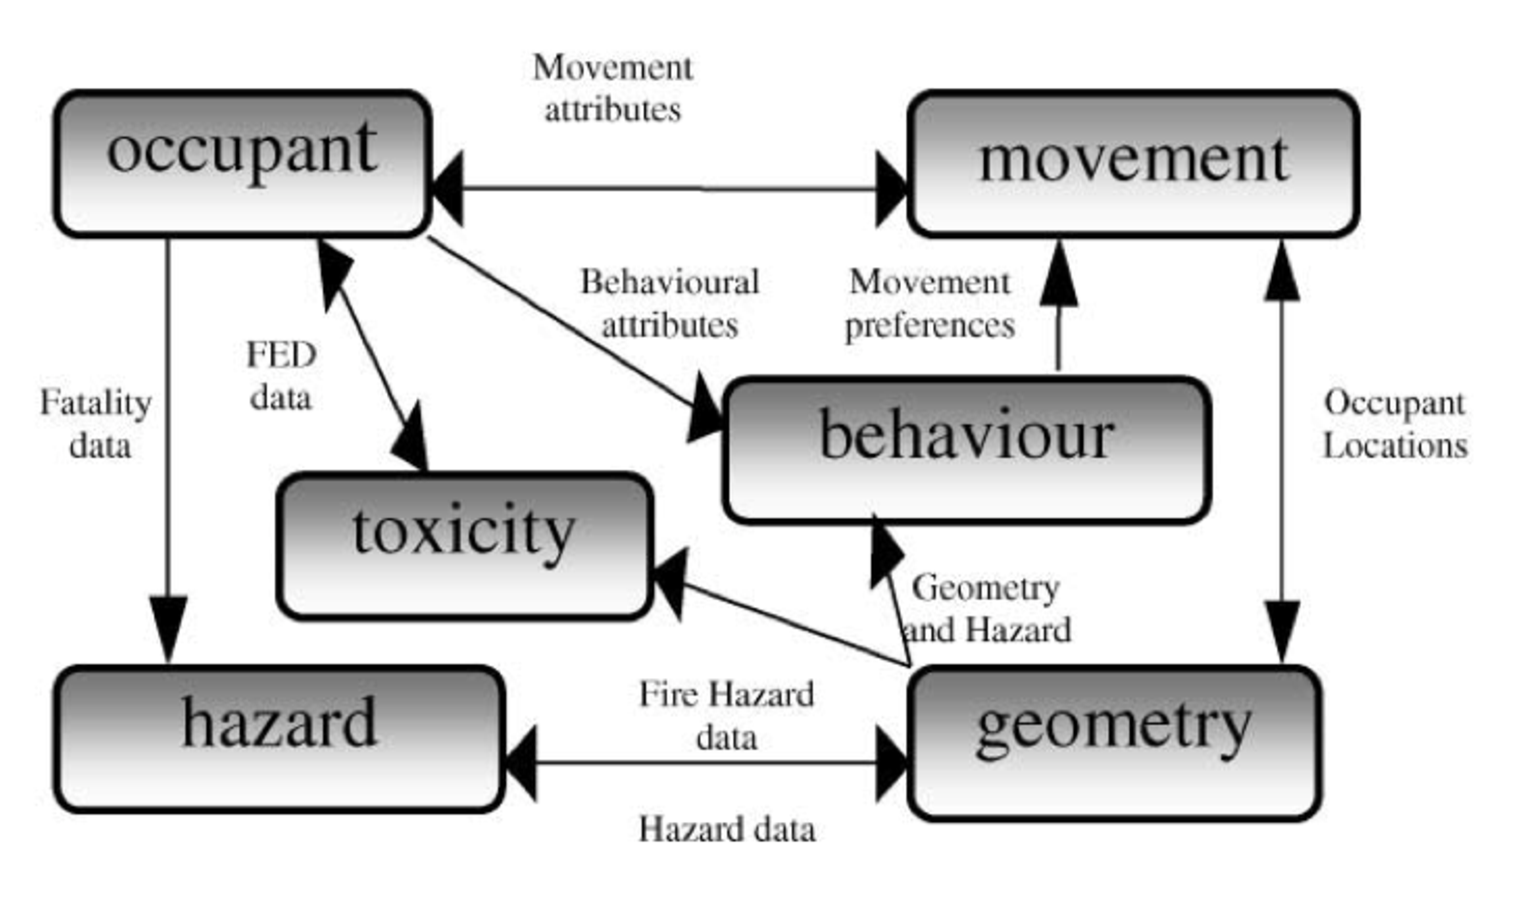
\includegraphics[width=\textwidth]{LiteratureReview/exodus}
\caption[EXODUS model]{Interaction of EXODUS modules~\cite{Gwynne:2001te}.}
\label{fig:ExodusDiagram}
\end{figure}


Once the building layout is specified as either a DXF file, CAD package, or by using the interactive tools provided in the suite, it is converted into a spatial grid representation which stores all the details of the building including obstacles present inside it. It is also able to store and show movement at staircases and across multiple levels. The grid itself is represented as a graph with the nodes representing a small region of space and each arc representing the distance between each node. Individuals travel from node to node along the arcs.

Each individual has more than 20 behavioral attributes that are specified at the start of the simulation and stored in the occupant submodule. Based on these, the behavioral module determines the behavior of the agents. Two kinds of behavior are modeled: \emph{normal} behavior and \emph{extreme} behavior. The only difference between the two is that in extreme behavior, the agents have a patience threshold beyond which they will stop queuing and resort to some other course of action. The behavior model works on two layers: a global layer and a local layer. The global layer gives a set of waypoints or a single destination~(possibly the exit or a familiar location). The local behavior is determined by the agent's attributes and determines factors like how long he waits before evacuating, conflict resolution and other things. Some of these factors and local behavior are probabilistically determined.

The toxicity submodule determines the physiological impact of the environment on the occupant. This submodule assumes that the effect of smoke or fire is determined by the dose received and not the exposure concentration. The toxicity affects the occupant's mobility agility and travel rates. The hazard module on the other hand is responsible for generating hazards like smoke and fire in the environment as a function of time and location. A dedicated zonal fire simulation model called CFAST is used for this purpose. Several analytics tools have also been developed to analyze the results produced by the simulations.

Gwynne et al.~\cite{Gwynne:2001te} added some new features including the ability to specify occupant specific knowledge of the layout of the building. The behavior module is further modified so that the agent chooses to use emergency exits that he knows of only when he is showing extreme behavior. This representation of a map of the place rather than just a path to exit allows the occupant to dynamically re-plan his route. He is also given the ability to learn from signs and through interactions with other agents.

The effect of smoke is also modeled by reducing the efficiency of the path selected and reducing the speed of movement as per the concentration of the smoke. This reduction in efficiency and speed happens only as long as the exit is not visible to the evacuee. A certain inertia in route replanning is also modeled to indicate the reluctance that people have in changing their pre-decided route.

Hollmann et al.~\cite{Hollmann:2010vy} presented a theoretical prototype of an emotional model that modeled the effect of time pressure and stress on evacuees was introduced into buildingEXODUS. Each agent is specified by giving a list of tasks or waypoints that he has to visit before or during the evacuation. The tasks are categorized as being compulsory, time critical and elective and each of them are given an estimated time for completion. An urgency factor indicates how constrained for time the agent perceives itself to be. The speed, drive, patience and the itinerary of each agent is rearranged based on the time elapsed, time left and the feelings of the person. Without an actual implementation of the prototype, it is difficult to analyze the strengths and weaknesses of the proposed emotional model.

The strength of EXODUS is the fact that it has a dedicated fire/ smoke simulation engine and a toxicity calculation module. The prototype of the emotion model to be used is also an innovative addition. The ability to specify so many parameters and thus the heterogeneity of agents is also important, as is the ability to model complex building layouts and obstacles in a variety of ways. Nevertheless, the model falls short on a few key factors. It does not try to model crowd behavior or its effects. The idea of cue perception and pre-evacuation behavior is very limited, unless the user specifies a list of tasks that each occupant is to do~\cite{Owen:1996jh}. However, the theoretical prototype for doing this was never implemented and tested.


\subsubsection{ESCAPES}

ESCAPES~\cite{Tsai:2011tz} is a multi agent based evacuation simulation software tailor-made for airport environments. Unlike most of the other models mentioned earlier, it also has a 3D visualization engine, which makes it more usable for security purposes for non experts. One of the ways in which this model improves on others is that it can model families and social bonds. It models how evacuees search for their family members before attempting to evacuate. Family members also communicate all their knowledge to other family members. It also models a fear factor and emotional contagion.  The knowledge of the fire spreads and the authority figures are able to calm people down. The model also takes into consideration the incomplete knowledge of most people and the spread of knowledge in the environment. However, the models for these are simplistic with only 2-3 states of fear, emotion and knowledge. The reaction time is modeled as a function of the proximity to the event. Agents that are near an event evacuate immediately, whereas others, will behave normally until they get enough information to know that they need to exit.

While the model includes some behavior like affiliation (within families), the prevalence of competitive behavior in the model is unrealistic. The family sizes are fixed~(Parents and two children) and the only social bonds that exist are within this family. The model of partial knowledge is rather simplistic as is the investigative behavior model. Despite these drawbacks, this is one of the few models that consider almost all the factors discussed in Section~\ref{LiteratureReview:PsychSummary}.

\subsubsection{MASSEgress}

Pan's~\cite{Pan:2006vp} multi agent based model of evacuation called MASSEgress is notable for the well structured and detailed architecture of the agents used and the importance that he gives to non-adaptive behavior being synonymous with a high stress evacuation environment.

Mobility, age, gender and body dimension are the only intrinsic characters that are included. A population generator is used to generate the required distribution of people based on these factors. The simulation uses a grid based physical environment which can be loaded as a CAD file. The data from simulation is logged to facilitate easy analysis, and a 2D and 3D visualization engine is also implemented for ease of use and simple analysis. The simulation engine itself simulates the behavior by dividing it into three parts: a perception engine, a behavior engine and a motor engine.

The perception model used is relatively complicated compared to the models discussed earlier. It consists of a point test method and a ray tracing algorithm implemented along with a visual cone. The visual cone specifies the region in which the agent can perceive and is determined by the eye position, viewing angle and visual range of the agents. The point test algorithm determines whether an exit or waypoint is perceived. The ray tracing algorithm determines which of the obstacles are perceived and ensures that only objects closest to the agent are perceived. modelling only the visual component of perception limits the model in certain ways that will be explored in more detail in Chapter~\ref{chapter:IBP}.

The agent behavior is considered to happen at three levels: an individual level, a group level and a crowd level. At the individual level, an agent generally acts using his experience. If experience can't help, they act rationally within the limits of their knowledge. If they are too stressed, then they start acting on \emph{instinct}. Instinct refers to competitive behavior where pushing, jumping out of windows and fleeing towards very crowded, blocked exits take place. At the interaction level, a social identity based model is used. Each agent has a social identity and each social identity has a set of actions associated with it. Depending on the situation, the actions taken by an agent are determined by the social identity. Pan assumes that during an extremely stressful situation people forget about their social roles. Personal spaces are defined for each individual which they always try to maintain. If this space is violated, they get agitated and stressed and will eventually lead to \emph{non-adaptive behavior}. The model also assumes a strong herding behavior, where the first reactors influence the reaction of the rest. At the crowd level, the three factors that influence the behavior of an agent are crowd density, environment constraints and perceived emotion and tension. The first two factors are standard in most crowd simulation environments. The third factor is interesting, it states how the individual's perception of a system as stressful determines how stressed he is, not just what happens to him. So even in a non emergency situation, \emph{non-adaptive behavior} might occur if a false alarm or some other stressful situation arises. Queuing, competitive, leader following, altruistic and herding behavior are modeled as resulting from the interaction of these different factors. A decision tree is used to simulate this behavior and to show how each of these behaviors is caused as a result of the aforementioned three levels. The actual implementation of the behavior at an individual level consists of 5 factors: familiarity~(memory), decision making type~(the intrinsic factors determined decision tree), urge to exit, stress threshold type and herding factor.

The movement engine has a simple collision detection algorithm and controls basic movements. Basic movement on stairways are also modeled.

The greatest strength of this model is the way in which the higher level behavior of agents are determined and described using a few fundamental lower level behaviors. It also has a more detailed visual perception system and movement system. However, it does not model pre-evacuation behavior or affiliative behavior of any sort. Like some of the other models, there is an undue prominence of non-adaptive behavior during evacuation.

\subsection{Summary}
\label{LiteratureReview:EngineeringSummary}
In this section, the different types of computational models of fires ranging from network based models to smart environments and agent based models were introduced. Seven existing models that model the key features highlighted in Section~\ref{LiteratureReview:PsychSummary} were also presented and analyzed.
\begin{itemize}
	\item Pires's model~\cite{Pires:2005gs} was one of the earliest to consider pre-evacuation behavior. However, the model abstracted away details of the pre-evacuation behavior as probabilities making it more difficult to study and analyze its effects.
	\item Still's thesis~\cite{Still:2000tp} highlighted the importance of data. He also, importantly, highlighted the fact it is not necessary to have a complicated model to simulate complex systems. Rather, simple rules may be able to produce the required complex behavior. Models should where possible follow Occam's razor, i.e.\ the simplest rules should be used. This was exemplified by Pan's MASSEgress model~\cite{Pan:2007gb} which produced higher level herding, following and competitive behavior by using simple lower level rules.
	\item Pelechano's work~\cite{Pelechano:2005vp} in combining a dedicated behavior model~(PMFServ) with their existing crowd simulation model~(MACES) demonstrated the importance of inter-disciplinary collaboration. By integrating an existing detailed emotion model to improve an existing computational model, they demonstrated the strengths and limitations of this approach.
	\item The Collective Panic Behavior Model~\cite{Franca:2009wq} demonstrated how a theory of human behavior can be computationally modeled without having to make any abstractions.
	\item The EXODUS model~\cite{Owen:1996jh} is one of the most detailed and mature models today. Hence, it is an excellent source of information on egress modelling and simulation.
    \item ESCAPES model~\cite{Tsai:2011tz} is significant for the importance given to modelling affiliative behavior and the spread of information.
	\item Pan's MASSEgress model~\cite{Pan:2006vp} despite not having the behavioral complexity of ESCAPES is notable for the structured approach to modelling agent behavior and it's ability to produce complex high level behavior using simple low level rules.
\end{itemize}

\section{Summary of Literature Review}
\label{LiteratureReview:Summary}
This chapter first introduced the complexity of the problem of modelling crowd evacuation and its multidisciplinary nature. In Section~\ref{LiteratureReview:CurrentUnderstanding}, the current theories on crowd behavior during an evacuation were presented. The salient features of human behavior during fire evacuation were identified from this and summarized in Section~\ref{LiteratureReview:PsychSummary}. In the following section, the different approaches to modelling crowds was introduced and some of the more significant models were presented in detail. Their strengths and shortcoming were summarized in Section~\ref{LiteratureReview:EngineeringSummary}.

 % Despite the variety and number of models available, there is still a lack of a detailed comprehensive model that takes into consideration the latest psychological and sociological theories of crowd behavior. Such a model needs to model the perception of cues and their interpretation; the uncertainty felt by evacuees at the beginning of an evacuation and their search for further information; their preference for familiarity and their search for affiliation and also the effects of stress and time constraints without resorting to the standard assumption of panic/ competitive behavior. In the following chapters, by leveraging on the strengths of existing computational models, a computational model for agents which models these behaviors is introduced.

This chapter has provided a broad overview of existing computational models of egress and briefly examined some of their strengths and weaknesses. Despite the number and variety of these models, several of the salient features of human behavior during egress identified in Section~\ref{LiteratureReview:CurrentUnderstanding} are generally ignored. At the same time, there exists similarities in the way behavior is generally modelled computationally. In the next chapter, the literature reviewed in the current chapter is used to identify the building blocks that make up a model of evacuee behavior. This helps in the identification of key research questions which are explored over the remainder of the thesis.

% THe following chapters then take each module at a time.

